\documentclass[a4paper,10pt]{article}
\usepackage[utf8]{inputenc}

% The following packages can be found on http:\\www.ctan.org
\usepackage{graphics} % for pdf, bitmapped graphics files
\usepackage{epsfig} % for postscript graphics files
\usepackage{mathptmx} % assumes new font selection scheme installed
\usepackage{times} % assumes new font selection scheme installed
\usepackage{amsmath} % assumes amsmath package installed
\usepackage{amssymb}  % assumes amsmath package installed
\usepackage{color, colortbl}

% define colors
\definecolor{Gray}{gray}{0.9}

%opening
\title{Essential Math Notes for Roboticists}
\author{
  Andreu Corominas-Murtra
  \thanks{
    Andreu Corominas-Murtra (andreu@beta-robots.com) is with Beta Robots (www.beta-robots.com) and IRI (www.iri.upc.edu).
    This notes are published under the Creative Commons License. In case of reference, please cite it as: Corominas-Murtra, A. Essential Math Notes for Roboticists. On-line at xxx. 2015. }
}

\begin{document}

\maketitle

\begin{abstract}
This document is a running collection of math notes. They try to summarize in a clear and useful way the math essentials for advanced robotics. The focus is put more on the interpretation of math entities and results, instead on computation and numerical recipes. The aim is to build a self reference tool for our daily work, and to share it. 
\end{abstract}

\newpage

\tableofcontents

\newpage
\section{Notation}
Main conventions and notation used through the document are listed below:

$a,b,c,x,y,z,u,v,w,...$ are scalars.

$\alpha,\beta,\theta,\phi$ are also scalars, by they usually represent angles. 

$\mathbf{a,b,c,x,y,z,o,p,r,u,v,w,...}$ are vectors.

$\mathbf{M,A,B,C,F,...}$ are matrices.

$\mathbf{R}$ is a rotation matrix.

$\mathbf{T}$ is a homogeneous transform matrix.

$\mathbf{I}_n$ is the identity matrix of dimensions $n \times n$.

$\mathcal{F}^C$ is the coordinate frame (shortly, frame) of body $C$.

$\mathbf{x}^C$ is a vector referenced with respect to the $\mathcal{F}^C$ coordinate frame.

$\mathbf{a}\in \mathbb{R}^3 \rightarrow \mathbf{a} = (a_x,a_y,a_z)^T$ are the components of a vector in 3D.

$\mathbf{a}^C_x$ is the first component of $\mathbf{a}$ expressed in frame~$\mathcal{F}^C$.

$i,j,k,l,.. \in \mathbb{Z}$ are usually running index over sets. 

$t \in \mathbb{Z}$ is usually an iteration index.

$\tau \in \mathbb{R}$ is usually a timestamp.

$\tau_t \in \mathbb{R}$ is the timestamp of iteration $t$.

$m,n,p,.. \in \mathbb{Z}$ are usually vector or matrix dimensions.

$p \in \mathbb{Z}$ is also used as a degree index of some function or polynomial. 

$\mathbf{q} = (q_r,q_x,q_y,q_z) = (a,b,c,d)$ is a quaternion. $q_r$ or~$a$ are the real parts.

$\hat{\mathbf{x}}$ is an estimate of $\mathbf{x}$, which is an actual (unknown) quantity.

\newpage

\section{Basic Trigonometry}
Trigonometry provides tools on the relations between angles and distance ratios in right triangles. 
Given the circle of unit radius ($r=1$) in figure~\ref{fig:trigonometry}, the cosine, sine and tangent are defined as: 
\begin{equation}
 \cos \alpha = \frac{a}{r} = \frac{a}{1} = a; \ \ \ \ 
 \sin \alpha = \frac{b}{r} = \frac{b}{1} = b; \ \ \ \ 
 \tan \alpha = \frac{b}{a};
\end{equation}
The above functions are defined as $f(\alpha):\mathbb{R} \rightarrow \mathbb{R}$. They are periodic functions with period $2\pi$, meaning that the function provides the same value for an argument $\alpha+k2\pi$,~being $k$ an integer ($k \in \mathbb{Z}$). 
\begin{figure}[bth!]
  \begin{center}
    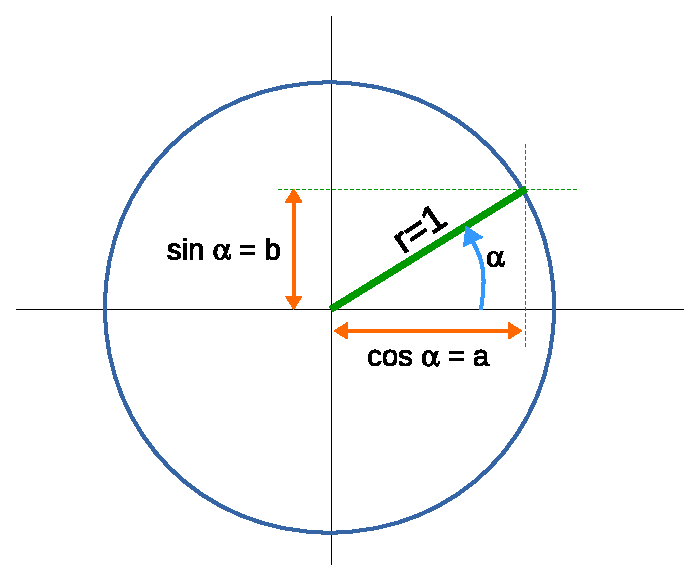
\includegraphics[width=1.0\columnwidth]{figures/trigonometry.eps}
    \caption{Unit circle and deifinitions of $\cos,\ \sin$ and~$\tan$. (to do)}
    \label{fig:trigonometry}
  \end{center}
\end{figure}

The inverse functions $acos(),\ asin()$ and~$atan()$ provides an angle given a ratio of distances. 

% \begin{minipage}[1pt]{c}
%  hello
% \end{minipage} 


\newpage

\section{Basic Algebra and Calculus}

\subsection{Functions}

A real \textbf{scalar function} defined in the $\mathbb{R}^n$ domain is:
\begin{equation}
 z=f(\mathbf{x}):\mathbb{R}^n \rightarrow \mathbb{R}, 
 \ \ z \in \mathbb{R}, \ \mathbf{x} \in \mathbb{R}^n.
\end{equation}

A real \textbf{vector function} defined in the $\mathbb{R}^n$ domain is:
\begin{equation}
 \mathbf{z}=f(\mathbf{x}):\mathbb{R}^n \rightarrow \mathbb{R}^m, 
 \ \ \mathbf{z} \in \mathbb{R}^m, \ \mathbf{x} \in \mathbb{R}^n.
\end{equation}

\subsection{Norm, dot and cross products }
\label{subsec:norm_dot_cross}

The \textbf{scalar or dot product} between two vectors is:
\begin{equation}
<\mathbf{u},\mathbf{v}> = \mathbf{u}^T \cdot \mathbf{v} = \mathbf{u}^T \mathbf{v} = \sum_{i=0}^{n-1} u_{i} v_{i}
, \ \ \mathbf{u},\mathbf{v} \in \mathbb{R}^n.
\end{equation}
The scalar product is a measure of the length of the projection of one vector over the axis of the other. 
Therefore, the scalar product can be also interpreted as a measure of similarity.

The $p$-\textbf{norm} of a vector is 
\begin{equation}
 \vert \mathbf{x} \vert _p = ( \sum_{i=0}^{n-1} x_{i}^p )^{\frac{1}{p}} \ .
\end{equation}
For $p = 2$, we found the \textbf{Euclidean norm}:
\begin{equation}
 \vert \mathbf{x} \vert _2 = \vert \mathbf{x} \vert = \sqrt{\sum_{i=0}^{n-1} x_{i}^2} = \mathbf{x}^T \mathbf{x}\ ,
\end{equation}
which is a measure of the length of $\mathbf{x}$, a fundamental concept.

If a vector is divided by its norm, $\frac{\mathbf{x}}{ \vert \mathbf{x} \vert }$ we obtain a \textbf{normalized} version, which can be interpreted as a vector of unit length pointing to the same direction of $\mathbf{x}$. Thus, normalized vectors indicate directions and lie on the hypersphere of unit radius. In 3D this can be interpreted as an \textbf{spherical projection}.

The scalar product between normalized $\mathbf{u}$ and $\mathbf{v}$ equals to the cosine of the angle between them:
\begin{equation}
 \frac{\mathbf{u}^T}{\vert \mathbf{u} \vert} \cdot \frac{\mathbf{v}}{\vert \mathbf{v} \vert} = 
 \frac{\mathbf{u}^T\mathbf{v}}{\vert \mathbf{u} \vert \vert \mathbf{v} \vert} =
 cos (\alpha) , \ \in [0,1]
\end{equation}
where $\alpha$ is the angle between vectors $\mathbf{u}$ and $\mathbf{v}$. This operation can be also interpreted as a similarity value between two normalized vectors. If normalized vectors are equal, the angle is 0, so the cosine is 1 (maximum similarity). Otherwise, if vectors are orthogonal, the angle is $\frac{\pi}{2}$, so the cosine results in 0 (minimum similarity). In the later case $\mathbf{u}$ and $\mathbf{v}$ span orthogonal directions. 

The \textbf{cross product} between two vectors is only defined in $\mathbb{R}^3$
\begin{equation}
 \mathbf{u} \times \mathbf{v} = \mathbf{w} , \ \ \mathbf{u},\mathbf{v},\mathbf{w} \in \mathbb{R}^3, 
\end{equation}
and results in a new vector $\mathbf{w}$ which is orthogonal to both $\mathbf{u}$ and $\mathbf{v}$. Components of the resulting vector are computed as: 
\begin{equation}
\mathbf{w} = 
\left[
\begin{array}{ccc}
  u_x\\
  u_y\\
  u_z\\
\end{array}
\right]
\times
\left[
\begin{array}{ccc}
  v_x\\
  v_y\\
  v_z\\
\end{array}
\right]
 = 
\left[
\begin{array}{ccc}
  u_y v_z - u_z v_y\\
  u_z v_x - u_x v_z\\
  u_x v_y - u_y v_x\\
\end{array}
\right]
 \end{equation}
Right hand rule, indicates forward direction of the resulting vector. That is, using the right hand, forefinger pointing as $u$, middle finger pointing following $v$, so the resulting $w$ is orthogonal to both, and points as thumb. 

\paragraph{Example \theexamplecounter. Code for norm, dot and cross products [C++/Eigen]}
\stepcounter{examplecounter}

% \begin{tcolorbox}
\begin{mdframed}
\begin{verbatim} 
#include eigen3/Eigen/Geometry 
 void main() 
 { 
    Eigen::Vector3d va; //va is a vector in R^3
    Eigen::Vector<double,3> vb; //vb is another vector in R^3
    va << 1,2,3; //fill the vector va
    vb << -1,-1,0; //fill the vector vb
    double norm_va = va.norm(); //|va|
    double dot_vab = va.dot(vb); //va^T · vb
    Eigen::Vector3d cross_vab = va.cross(vb);//va x vb 
 }  
\end{verbatim}
\end{mdframed}


\subsection{Matrix Manipulation}
A \textbf{matrix} is a rectangular array of numbers, so they are sorted in rows and columns:
\begin{equation}
\mathbf{A} \in \mathbb{R}^{m \times n}
\left[
\begin{array}{ccccc}
  a_{00} & \dots & a_{0j} & \dots & a_{0n-1} \\
  a_{10} & \dots & \dots & \dots & a_{1n-1} \\
  \dots & \dots & \dots & \dots & \dots \\
  a_{i0} & \dots & a_{ij} & \dots & a_{in-1} \\
  \dots & \dots & \dots & \dots & \dots \\
  a_{m-10} & \dots & a_{m-1j} & \dots & a_{m-1n-1} \\
\end{array}
\right]
\end{equation}
A matrix lies on a $\mathbb{R}^{m \times n}$ space, where the dimensions are the number of rows $m$, and the number of columns $n$. Element $a_{ij}$ represents a generic element of the matrix $\mathbf{A}$. Matrices are usually interpreted as a set of column or row vectors: a set of $m$ row vectors of dimension $n$, or a set of $n$ column vectors of dimension $m$. Following this interpretation, it can be written: 
\begin{equation}
\mathbf{A} = 
\left[
\begin{array}{c}
  \bar{\mathbf{a}}_0 \\
  \bar{\mathbf{a}}_1 \\
  \dots \\
  \bar{\mathbf{a}}_i \\
  \dots \\
  \bar{\mathbf{a}}_{m-1} \\
\end{array}
\right]
 = 
\left[
\begin{array}{ccccc}
  \mathbf{a}_0 & \dots & \mathbf{a}_j & \dots & \mathbf{a}_{n-1} \\
\end{array}
\right], 
\end{equation}
where $\bar{\mathbf{a}}_i$ means the row vector corresponding to row $i$. 

A matrix is called \textbf{squared} when $n=m$.

A matrix is called \textbf{diagonal} when $a_{ij}=0, \forall i\neq j$, and $a_{ij}\neq0, \forall i=j$

A matrix is called \textbf{orthogonal} when its rows or columns are orthogonal vectors, which can be checked if their scalar product is zero.  

A matrix is called \textbf{upper triangular} when $a_{ij}=0, \forall i>j$, and \textbf{lower triangular} when $a_{ij}=0, \forall i<j$.

$\mathbf{I}_n$ is the identity matrix, which is a diagonal matrix with all non-zero elements set to 1. 

The \textbf{sum} of two matrix is done element by element, so both matrix should have the same dimensions, as well as the resulting matrix:
\begin{equation}
\mathbf{A} = \mathbf{B} + \mathbf{C}, \ \mathbf{A}, \mathbf{B}, \mathbf{C} \in \mathbb{R}^{m \times n} \ \rightarrow a_{ij} = b_{ij} + c_{ij}
\end{equation}

The matrix \textbf{product}
\begin{equation}
\mathbf{A} = \mathbf{B}\ \mathbf{C}, \ 
\mathbf{A} \in \mathbb{R}^{m \times n }, 
\mathbf{B} \in \mathbb{R}^{m \times p }, 
\mathbf{C} \in \mathbb{R}^{p \times n }
\label{eq:mat_product}
\end{equation}
is computed as follows: 
\begin{equation}
a_{ij} = \bar{\mathbf{b}}_i \cdot \mathbf{c}_j = \sum_{i=0}^{p-1} b_{ip} c_{pj}. 
\end{equation}
Each resulting component can be viewed as a scalar product between $\bar{\mathbf{b}}_i$ and $\mathbf{c}_j$, 
so all comments exposed above regarding the scalar product can be interpreted for the matrix product. Please note in equation~\ref{eq:mat_product} matrix dimensions of $\mathbf{B}$ and $\mathbf{C}$, and the resulting dimensions of $\mathbf{A}$. Matrix multiplication is allowed if and only if the number of columns of the first operand is equal to the number of rows of the second operand. Therefore, matrix multiplication is not a commutative operation in a general case. 

The \textbf{rank} of a matrix is the minimum between the number of independent rows and the number of independent columns. An independent vector (row or column) means that it cannot be expressed as a linear combination of the other vectors (rows or columns) of the matrix. Therefore an independent vector adds a new dimension to the space the vectors of the matrix are spanning. 

The \textbf{matrix determinant} is defined for squared matrices, and it is computed following this recursive expression: 
\begin{equation}
det(\mathbf{A}) = |\mathbf{A}| = \sum_{j=0..n-1} (-1)^{1+j}\ a_{ij}\ det(\mathbf{A}_{-0j})
\end{equation}
where $\mathbf{A}_{-0j}$ is the matrix composed by $\mathbf{A}$ but removing its first row and column~$j$. For $n=2$ this expression is reduced to:  
\begin{equation}
\left|
\begin{array}{cc}
  a_{00} & a_{01}\\
  a_{10} & a_{11} \\
\end{array}
\right| = 
a_{00}a_{11} - a_{01}a_{10}
\end{equation}
A matrix is called rank deficient or null-rank when its determinant is zero, meaning that some row or column can be expressed as a linear combination of other rows or columns respectively.

The determinant is a measure of the hypervolume of the hyperellipsoide represented by matrix $\mathbf{A}$. 

% \paragraph{Example~\ref{par:ex_determinant}}
% \label{par:ex_determinant}
% %Deteriminant as a measure of hipervolume, eigen vectors as the direction of ellipses major and minor axis, 
% Let's see an example in 2D, where the hypervolume becomes the area. Given the matrix
% \begin{equation}
% \mathbf{A} = 
% \left|
% \begin{array}{cc}
%   1.5 & 0.5\\
%   0.5 & 2 \\
% \end{array}
% \right|
% \end{equation}
% which could be the resulting covariance matrix from some estimation process. We want to visualize what the determinant is showing, so we compute it: 
% \begin{equation}
%  |\mathbf{A}| = 1.5 \cdot 2 - 0.5 \cdot 0.5 = 2.75
% \end{equation}


The \textbf{transpose} of~$\mathbf{A}$, only defined for squared matrices, is~$\mathbf{A}^T$, where its elements exchange columns by rows: 
\begin{equation}
 \mathbf{A} = \{a_{ij}\}; \ \mathbf{A}^T =\{a_{ji}\} 
\end{equation}


Given a squared matrix~$\mathbf{A}$ of sizes $n \times n$, $\mathbf{A}^{-1}$ is the \textbf{inverse} of a $\mathbf{A}$, so it fulfills that $\mathbf{A}^{-1}$ is also squared $n \times n$ and:
\begin{equation}
 \mathbf{A}\mathbf{A}^{-1} = \mathbf{A}^{-1}\mathbf{A} = \mathbf{I}_n
\end{equation}

The following is a list of useful expressions~\cite{henderson80}, [...]: 
\begin{align}
 (\mathbf{A}^{-1})^{-1} & = \mathbf{A} \\
 (\mathbf{A}^T)^{-1} & = (\mathbf{A}^{-1})^T \\
 (a \mathbf{A})^{-1} & = a^{-1} \mathbf{A}^{-1}\\
 (\mathbf{A}\mathbf{B})^T & = \mathbf{B}^T\mathbf{A}^T\\
 (\mathbf{A}\mathbf{B})^{-1} & = \mathbf{B}^{-1}\mathbf{A}^{-1}\\
 \mathbf{A}(\mathbf{B}+\mathbf{C}) & = \mathbf{A}\mathbf{B}+\mathbf{A}\mathbf{C}\\ 
 (\mathbf{A}+\mathbf{B})^T & = \mathbf{A}^T + \mathbf{B}^T\\
 (\mathbf{A}+\mathbf{B})^{-1} & = \mathbf{A}^{-1}-\mathbf{A}^{-1}\mathbf{B}(\mathbf{I}+\mathbf{A}^{-1}\mathbf{B})^{-1}\mathbf{A}^{-1}
\end{align} 

The following equation shows the \textbf{matrix inversion lemma}. It's a useful expression in situations where matrix $\mathbf{A}$ and~$\mathbf{C}$ are easy to invert, because they may be diagonal or have small dimension. In such case it can be applied:
\begin{equation}
 (\mathbf{A}+\mathbf{B}\mathbf{C}\mathbf{D})^{-1} = 
  \mathbf{A}^{-1}-\mathbf{A}^{-1}\mathbf{B}\mathbf{C}(\mathbf{C}+\mathbf{C}\mathbf{D}\mathbf{A}^{-1}\mathbf{B}\mathbf{C})^{-1}
  \mathbf{C}\mathbf{D}\mathbf{A}^{-1}
\end{equation}
The prove can be found at[ref], but it starts by multiplying at each side by $(\mathbf{A}+\mathbf{B}\mathbf{C}\mathbf{D})$.

The \textbf{skew-symmetric matrix} in $\mathbb{R}^3$ is defined as a square matrix whose transpose is also its negative:
\begin{equation}
\mathbf{A} = 
\left[
\begin{array}{ccc}
  0 & a & -b\\
  -a & 0 & c\\
  b & -c & 0\\
\end{array}
\right].
\end{equation}
The skew matrix can be useful to represent the vector product as a matrix-vector product. If $\mathbf{a}=[a_x,a_y,a_z]$ is a vector in $\mathbb{R}^3$, let be $\mathbf{A}$ the following matrix:
\begin{equation}
\mathbf{A}_s(\mathbf{a}) = \mathbf{A}_s 
\left[
\begin{array}{ccc}
  0 & -a_z & a_y\\
  a_z & 0 & -a_x\\
  -a_y & a_x & 0\\
\end{array}
\right], 
\end{equation}
then the vector product of $\mathbf{a}\times\mathbf{b}$ can be expressed as:
\begin{equation}
 \mathbf{a}\times\mathbf{b} = \mathbf{A}_s\mathbf{b} 
\end{equation}
A \textbf{hermitian} matrix is that fulfilling: 
\begin{itemize}
 \item $\mathbf{A}$ is square $n\times n$.
 \item $\mathbf{A} = (\mathbf{A}^T)^* \rightarrow a_{ij} = a_{ji}^*$
\end{itemize}
And a \textbf{positive-definite} matrix is that fulfilling: 
\begin{itemize}
 \item $\mathbf{A}$ is square $n\times n$.
 \item $\mathbf{v}^T\mathbf{A}\mathbf{v} > 0, \ \forall\mathbf{v}\in \mathbb{R}^n$, and $\neq \mathbf{0} $.
\end{itemize}
Both later cases are commonly found in practical robotics applications and present interesting properties exploited by algebra programming libraries.


\newpage

\section{Rigid Transformations}

Rigid transformations is a major topic in robotics. From perception, to kinematics and control, everywhere the concept of a rigid transformation appears. A rigid transformation defines the rotation and translation between two coordinate frames. How  both this translation, and specially this rotation, are represented (or parameterized) introduce fundamental concepts reviewed in the following paragraphes. 

Coordinate frames will be written as $\mathcal{F}^A,\ \mathcal{F}^B$, for frames~$A$ and~$B$. They could be positioned, for instance, at the pivot point of a platform and at the center point of a sensor.  

\subsection{Rotations}
There are several ways to represent a rotation. The most used ones are the following: rotation matrix, quaternion, Euler angles and axis angle. Each representation has benefits and drawbacks, depending on the application. For instance, for a sea ship which will never flip (hopefully), Euler angles could be a good option, but for an end effector tool expected to cover all orientations in 3D, quaternions or Rotation matrix could be better. 

\subsubsection{Rotation Matrix}
\label{subsec:rotation_matrix}
\paragraph{Definition} A rotation matrix~$\mathbf{R}$ is a squared, orthogonal matrix with $|\mathbf{R}|=1$. 

\paragraph{Interpretation} Columns of $\mathbf{R}$ can be interpreted as orthonormal vectors expressing a frame~$\mathcal{F}^B$ in terms of another frame~$\mathcal{F}^A$. In that case, such rotation matrix is expressed as~$\mathbf{R}^A_B$. Given two frames which are rotated, $\mathcal{F}^A$ and~$\mathcal{F}^B$, and given a vector~$\mathbf{v}^B$ expressed in terms of~$\mathcal{F}^B$, the following equation expresses the vector~$\mathbf{v}$ with its new coordinates in terms of~$\mathcal{F}^A$:
\begin{equation}
 \mathbf{v}^A = \mathbf{R}^A_B \mathbf{v}^B
\end{equation}
It fulfills also 
\begin{equation}
 \mathbf{v}^B = (\mathbf{R}^A_B)^{-1} \mathbf{v}^A = \mathbf{R}^B_A \mathbf{v}^A
\end{equation}

The number of parameters required for this parameterization is $n \times n$ in an $n$-dimension space. In 3D, for instance, 9 numbers are required. However, these 9 parameters have to fulfill certain conditions between them, so they are not free. These conditions are imposed by the definition of the rotation matrix itself: orthogonality and unit determinant.  

\paragraph{Chain of Rotations}
If a third frame~$\mathcal{F}^C$ is also rotated with respect to frame~$\mathcal{F}^B$, then the equation representing the chain of rotations, from a point expressed in terms of~$\mathcal{F}^C$ to the point expressed in terms of~$\mathcal{F}^A$, is: 
\begin{equation}
 \mathbf{v}^A = \mathbf{R}^A_B \mathbf{R}^B_C \mathbf{v}^C = \mathbf{R}^A_C \mathbf{v}^C
\end{equation}
Please be careful with the sequence of the matrix product representing the chain, since matrices are ordered from right to left, starting from the \textit{outer} rotation up to the \textit{inner} one. In the 3D case, computing~$\mathbf{R}^A_C$ requires 27 multiplications and 18 additions. 


\paragraph{Example \theexamplecounter. Rotations in 2D}
\stepcounter{examplecounter}
In 2D, if frame~$\mathcal{F}^B$ is rotated by~$\alpha=30^o$ degrees with respect to frame~$\mathcal{F}^A$, the matrix representing this rotation is as follows: 
\begin{equation}
\mathbf{R}^A_B = 
\left[
\begin{array}{cc}
  \cos\alpha & -\sin\alpha\\
  \sin\alpha & \cos\alpha\\
\end{array}
\right] = 
\left[
\begin{array}{cc}
  \frac{\sqrt{3}}{2} & -\frac{1}{2}\\
  \frac{1}{2} & \frac{\sqrt{3}}{2}\\
\end{array}
\right] 
\end{equation}
Given $\mathbf{v}^B = [2\ 1]^T$ a vector (point) represented in terms of frame~$\mathcal{F}^B$, its coordinates in terms of frame~$\mathcal{F}^A$ are:
\begin{equation}
 \mathbf{v}^A = \mathbf{R}^A_B \mathbf{v}^B =
\left[
\begin{array}{cc}
  \frac{\sqrt{3}}{2} & -\frac{1}{2}\\
  \frac{1}{2} & \frac{\sqrt{3}}{2}\\
\end{array}
\right]
\left[
\begin{array}{c}
 2 \\
 1\\
\end{array}
\right] =
\left[
\begin{array}{c}
 1.232 \\
 1.866\\
\end{array}
\right]
\end{equation}
so $\mathbf{v}^A=[1.232\ 1.866]^T$ is the same point $\mathbf{v}$ but expressed in terms of frame~$\mathcal{F}^A$.


\subsubsection{Quaternions}
\paragraph{Definition} A quaternion[ref] is an extension of Complex numbers to 3D. As complex numbers can be represented as vectors in $\mathbb{R}^2$, quaternions can be represented as vectors in~$\mathbb{R}^4$, with one real part,~$a$, and three imaginary parts,~$b,c,d$: 
\begin{equation}
 \mathbf{q} = [q_r\ q_i\ q_j\ q_k]^T = 
    q_r\mathbf{1} + q_i\mathbf{i} + q_j\mathbf{j} + q_k\mathbf{k}=
    q_r + q_i\mathbf{i} + q_j\mathbf{j} + q_k\mathbf{k}, 
\end{equation}
so quaterions are defined over a base formed by vectors $\mathbf{1},\mathbf{i},\mathbf{j},\mathbf{k}$. Definition of this base is required to define the quaternion product. Vectors of this base fulfill:
\begin{itemize}
 \item $\mathbf{1}$ is the identity element $\rightarrow\ \mathbf{q}\mathbf{1} = \mathbf{q}$
 \item $\mathbf{i}\mathbf{i}=\mathbf{j}\mathbf{j}=\mathbf{k}\mathbf{k}=\mathbf{i}\mathbf{j}\mathbf{k}=-1$
 \item $\mathbf{i}\mathbf{j}=\mathbf{k};\ \mathbf{j}\mathbf{k}=\mathbf{i};\ \mathbf{k}\mathbf{i}=\mathbf{j};$
\end{itemize}

The \textbf{sum} of two quaternions, $\mathbf{q}^a$ and $\mathbf{q}^b$, is defined as the sum in $\mathbb{R}^4$:
\begin{equation}
 \mathbf{q} = \mathbf{q}^a + \mathbf{q}^b = [ (q^a_r+q^b_r)\ 
					      (q^a_i+q^b_i)\ 
					      (q^a_j+q^b_j)\
					      (q^a_k+q^b_k)\ ]^T
\end{equation}
and the \textbf{scalar product} of a quaternion is:
\begin{equation}
 u\mathbf{q} = [ uq_r\ uq_i\ uq_j\ uq_k]^T, \ \ u \in \mathbb{R}, 
\end{equation}
which also coincides with the scalar product in $\mathbb{R}^4$.

However, the \textbf{quaternion product} is quite more different than what we do with vectors in~$\mathbb{R}^4$. We use here the properties of the base $\{\mathbf{1,i,j,k}\}$ defined above, and the distributive law: 
\begin{equation}
 \mathbf{q} = \mathbf{q}^a \cdot \mathbf{q}^b =
 \left[
 \begin{array}{c}
    q^a_rq^b_r - q^a_iq^b_i - q^a_jq^b_j - q^a_kq^b_k\\
    q^a_rq^b_i + q^a_iq^b_r + q^a_jq^b_k - q^a_kq^b_j\\
    q^a_rq^b_j - q^a_iq^b_k + q^a_jq^b_r + q^a_kq^b_i\\
    q^a_rq^b_k + q^a_iq^b_j - q^a_jq^b_i + q^a_kq^b_r\\
 \end{array}
 \right]. 
%      m_aux = [p(1) -p(2) -p(3) -p(4); p(2:4) ( p(1)*eye(3,3) + skewMatrix(p(2:4)))];
%     q_out = m_aux*q;
\end{equation}

Finally, the \textbf{conjugate} of a quaternion is denoted as $\mathbf{q}^*$ and is computed as:
\begin{equation}
 \mathbf{q}^* = [q_r\ -q_i\ -q_j\ -q_k]^T
\end{equation}


\paragraph{Definition} \textbf{Unit quaternions} are those with unit norm,~$|\mathbf{q}|=1$. They are a way to represent rotations in 3D, usually not so intuitive, but with major practical benefits, specially in computer implementations. Let be a quaternion $\mathbf{q}^A_B$ a quaternion representing the rotation of frame~$\mathcal{F}^B$ with respect to frame~$\mathcal{F}^A$. Then, given a vector $\mathbf{v}^B$ expressed in terms of~$\mathcal{F}^B$, its components in terms of~$\mathcal{F}^A$ can be computed with the following equation: 
\begin{equation}
\left[
 \begin{array}{c}
 0\\
 v^A_x\\
 v^A_y\\
 v^A_z\\
 \end{array}
 \right] 
 =
 \mathbf{q}^A_B
 \cdot
 \left[
 \begin{array}{c}
 0\\
 v^B_x\\
 v^B_y\\
 v^B_z\\
 \end{array}
 \right]
 \cdot
 (\mathbf{q}^A_B)^*
\end{equation}
where the two product involved in the right side of the equation are quaternion products.  

\paragraph{Interpretation}
A good way to interpret 3D rotations represented by unit quaternions is to revisit how Complex numbers can represent 2D rotations. Let $\mathbf{c}=a+bi\ \in\mathbb{C}$ be a complex number with unit norm, $|\mathbf{c}|=1$. In that case, $\mathbf{c}$ is representing a point in the unit circle lying on the 2D plane, so it is also representing an angle $\alpha$ (FigureXX). This complex number can be written as:
\begin{equation}
 \mathbf{c} = \cos\alpha + \sin\alpha i
\end{equation}
Quaternions are an extension of this idea but exported to 3D, so they require three imaginary parts to fully represent a rotation, instead of a single imaginary part required in 2D:
\begin{equation}
 \mathbf{q} = \cos\frac{\alpha}{2} + u_x\sin\frac{\alpha}{2} \mathbf{i} + u_y\sin\frac{\alpha}{2} \mathbf{j} + u_z\sin\frac{\alpha}{2} \mathbf{k}
\end{equation}
where $\alpha$ is the angle over the rotation axis indicated by the vector $\mathbf{u}=[u_x\ u_y\ u_z]^T$. Therefore, if we rotate a vector over the Euclidean $X,Y$ or~$Z$ axes, we get a complex representations over each $x=0,y=0$ or~$z=0$ planes respectively. 

\paragraph{Chain of Rotations}
Unit quaternions behave very similarly to rotation matrix when chaining rotations. Lets involve three frames~$\mathcal{F}^A$,~$\mathcal{F}^B$ and~$\mathcal{F}^C$. $\mathbf{q}^A_B$ represents the rotation of frame~$B$ with respect to frame~$A$, and $\mathbf{q}^B_C$ represents the one of frame~$C$ with respect to~$B$. Then, $\mathbf{q}^A_C$, which is the rotation of frame~$C$ with respect to~$A$ is:
\begin{equation}
 \mathbf{q}^A_C = \mathbf{q}^A_B \cdot \mathbf{q}^B_C
\end{equation}
The operation required to compute~$\mathbf{q}^A_C$ performs 16 multiplications and 12 additions, so it is more computationally efficient than matrix chaining. This can be of relevance in real-time algorithms requiring massive computtaion of chains of rotations.

\paragraph{Conversion to Rotation Matrix}
Sometimes it can be useful to convert a quaternion to a rotation matrix. The formula below provides such conversion: 
\begin{equation}
\mathbf{R}(\mathbf{q}) = 2
\left[
\begin{array}{ccc}
\frac{1}{2} - q^2_2 - q^2_3 & q_1q_2-q_0q_3 & q_0q_2+q_1q_3 \\

q_0q_3+q_1q_2 & \frac{1}{2} - q^2_1 - q^2_3 &   q_2q_3-q_0q_1\\

q_1q_3-q_0q_2 & q_0q_1+q_2q_3 & \frac{1}{2} - q^2_1 - q^2_2
\end{array}
\right],
\end{equation}


\subsubsection{Axis Angle}
//TODO

\subsubsection{Euler Angles}
\paragraph{Definition}
Euler angles approach is an intuitive way to represent rotations, by expressing the three rotation angles applied to different orthogonal axis, in a given order. One of the most used conventions is the $Z-Y-X$ order, leading to three angles:
\begin{itemize}
  \item	Yaw, $\theta$, is the first angle, a rotation around the $Z$ axis of the reference frame, $\theta \in (-\pi, \pi]$.
  \item Pitch, $\phi$, is the second angle, a rotation around the current (once rotated) $Y$ axis, $\phi \in (-\pi/2, \pi/2]$.
  \item Roll, $\psi$, is the third angle, a rotation around the current (twice rotated) $X$ axis, $\psi \in (-\pi, \pi]$.
\end{itemize}
Figure~\ref{appF:fig:threeAngles} shows the order of the rotations of each euler angle to get the final orientation.
\begin{figure}[h]
\centering
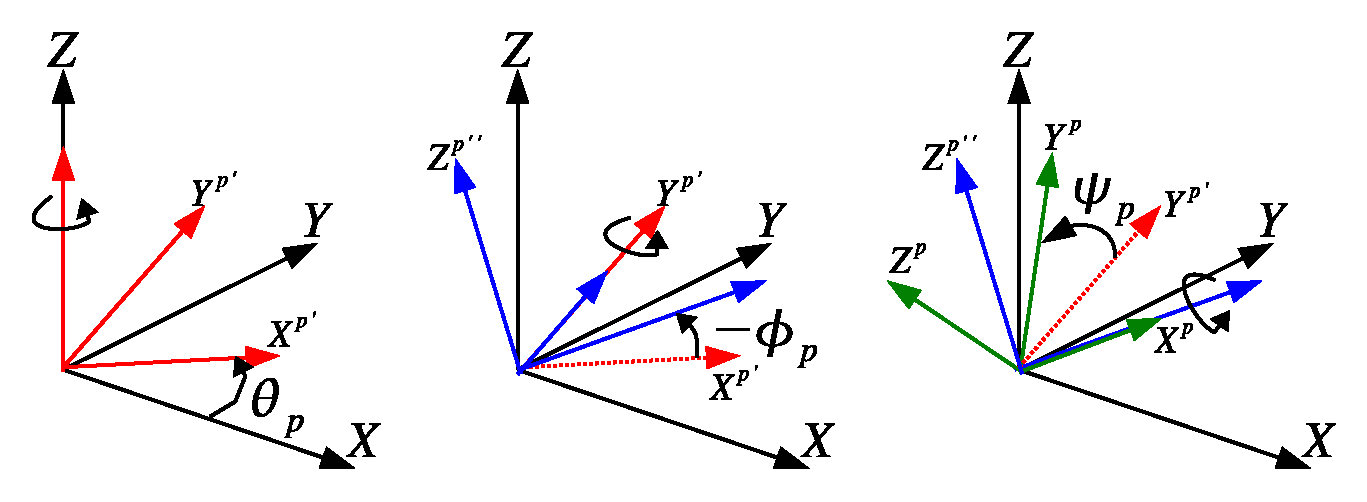
\includegraphics[height=4.2cm]{figures/threeAngles.eps}
\caption{Definition of the three euler angles yaw ($\theta$), pitch ($\phi$) and roll ($\psi$). Reference frame drawn in black. Intermediate frames drawn in red and blue. Final orientation frame shown in green. }
\label{appF:fig:threeAngles}
\end{figure}

\paragraph{Conversion to Rotation Matrix}
Since rotations are performed always around the current axis instead of around the fixed world axis, the whole rotation matrix is computed as:
\begin{equation}
 R(\theta,\phi,\psi) = R_{\theta,\phi,\psi} = R_z(\theta)R_y(\phi)R_x(\psi)
\end{equation}
where,
% //TODO: reedit matriz with [] style. And fit all in a single ``row''
%\begin{scriptsize}
\begin{equation}
\begin{split}
 & R_z(\theta)=
\begin{pmatrix}
 \cos\theta  & -\sin\theta & 0 \\
 \sin\theta & \cos\theta & 0 \\
 0          & 0         & 1 \\
\end{pmatrix}; \\
%\end{equation}
%\begin{equation}
%\label{appF:eq:R2} 
 & R_y(\phi)=
\begin{pmatrix}
 \cos\phi  & 0 & -\sin\phi \\
 0	    & 1	& 0 \\
 \sin\phi  & 0 & \cos\phi \\
\end{pmatrix};\\
%\end{equation}
%\begin{equation}
%\label{appF:eq:R3} 
 & R_x(\psi)=
\begin{pmatrix}
 1	       & 0 	& 0 \\
 0 & \cos\psi & -\sin\psi \\
 0 & \sin\psi & \cos\psi \\
\end{pmatrix};\\
\end{split}
\label{appF:eq:R123} 
\end{equation}
%\end{scriptsize}


\subsection{Adding translation}
Beyond rotations, a transformation may involve also a translation, which is the displacement between two frames, without taking into account their orientation. If two frames are translated, there is simply a vector to add between them: 
\begin{equation}
 \mathbf{v}^A = \mathbf{v}^B + \mathbf{p}^A_B
\end{equation}
where $\mathbf{p}^A_B$ is the vector expressing central point of frame~$B$ in terms of frame~$A$. 

When frame~$B$ is both rotated and translated with respect to frame~$A$, we apply first the rotation, and then the translation (see Figure~\ref{fig:rotation_translation}):
\begin{equation}
 \mathbf{v}^A = \mathbf{R}^A_B\mathbf{v}^B + \mathbf{p}^A_B
\end{equation}
\begin{figure}[bth!]
  \begin{center}
    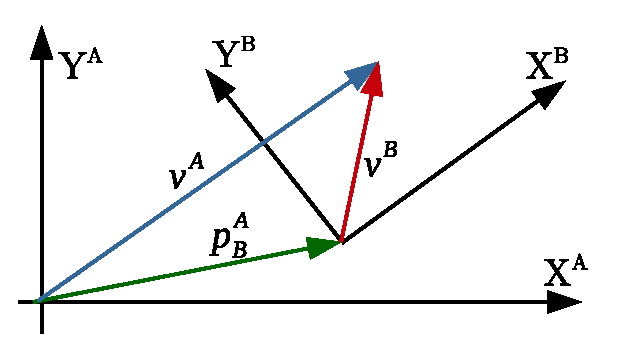
\includegraphics[width=0.8\columnwidth]{figures/rotation_translation.eps}
    \caption{A frame B, rotated and translated with respect to frame A.}
    \label{fig:rotation_translation}
  \end{center}
\end{figure}



\subsection{Homogeneous matrix}
\label{subsec:homogeneous_matrix}
Homogeneous matrix is a compact way to represent both rotation and translation in a single matrix, by adding an extra dimensionality to the rotation matrix.  
The homogeneous matrix representing the frame~$B$ in terms of the frame~$A$ (both rotation and translation) is defined as:
\begin{equation}
 \mathbf{T}^A_B = 
 \left[
 \begin{array}{cc}
  \mathbf{R}^A_B & \mathbf{p}^A_B \\
  0	& 	1 \\
 \end{array}
\right]
\end{equation}
Then, as it was described by pure rotation case in subsection~\ref{subsec:rotation_matrix}, it fulfills that:
\begin{equation}
\left[
 \begin{array}{c}
  \mathbf{v}^A \\
  1
 \end{array}
 \right]
 = \mathbf{T}^A_B 
 \left[
 \begin{array}{c}
  \mathbf{v}^B \\
  1
 \end{array}
 \right]; \ \
 \left[
 \begin{array}{c}
  \mathbf{v}^B \\
  1
 \end{array}
 \right]
  = (\mathbf{T}^A_B)^{-1} 
 \left[
 \begin{array}{c}
  \mathbf{v}^A \\
  1
 \end{array}
 \right].
\end{equation}
Homogeneous matrixes also allow chaining as rotations do:
\begin{equation}
 \left[
 \begin{array}{c}
  \mathbf{v}^A \\
  1
 \end{array}
 \right]
 = \mathbf{T}^A_B \mathbf{T}^B_C 
  \left[
 \begin{array}{c}
  \mathbf{v}^C \\
  1
 \end{array}
 \right]
 = \mathbf{T}^A_C 
  \left[
 \begin{array}{c}
  \mathbf{v}^C \\
  1
 \end{array}
 \right].
\end{equation}

\paragraph{Example \theexamplecounter. Vehicle frames.}
%\label{example:vehicle_frames}
\stepcounter{examplecounter}
As Figure~\ref{fig:world_vehicle_sensor_frames} draws, imagine we have a vehicle well localized at point $p^O=\left[p^O_x\ p^O_y\right]^T$ and oriented an angle~$\theta$ with respect to the origin of the trajectory. This vehicle has a sensor mounted at the known position~$m^B=[m^B_x\ m^B_y]$ and oriented an angle~$\beta$ with respect to the base frame of the vehicle. Finally this sensor has detected a point of interest at~$q^S=[q^S_x\ q^S_y]$. Which are the coordinates of the point of interest with respect to the base frame, and with respect to the origin of the trajectory ?
\begin{figure}[bth!]
  \begin{center}
    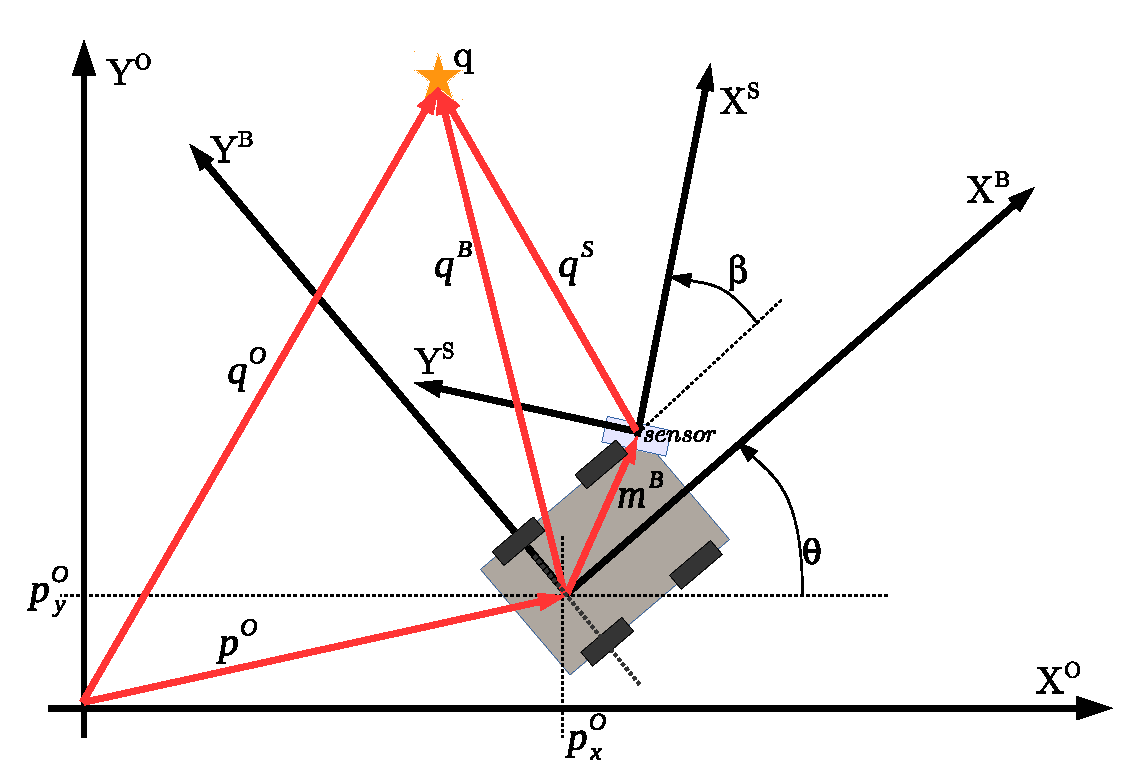
\includegraphics[width=1.0\columnwidth]{figures/world_vehicle_sensor_frames.eps}
    \caption{Trajectory, vehicle and sensor frames.}
    \label{fig:world_vehicle_sensor_frames}
  \end{center}
\end{figure}

The rotation matrixes involved are:
\begin{equation}
\mathbf{R}^O_B = 
\left[
 \begin{array}{cc}
    cos\theta   &  -sin\theta  \\
    sin\theta  & cos\theta \\
 \end{array}
 \right];\ \ 
\mathbf{R}^B_S = 
\left[
 \begin{array}{cc}
    cos\beta   &  -sin\beta  \\
    sin\beta  & cos\beta \\
 \end{array}
 \right];\ \ 
\end{equation}
and the homogeneous matrixes representing the transformations from the origin to the base, and from the base to the sensor, are respectively:
\begin{equation}
\mathbf{T}^O_B = 
\left[
 \begin{array}{cc}
    \mathbf{R}^O_B  &  p^0  \\
    \mathbf{0} & 1 \\
 \end{array}
 \right];\ \ 
\mathbf{T}^B_S = 
\left[
 \begin{array}{cc}
    \mathbf{R}^B_S  &  m^B  \\
    \mathbf{0} & 1 \\
 \end{array}
 \right];\ \ 
\end{equation}
So the point~$q$ with respect to the vehicle base frame and with respect to the origin of the trajectory is: 
\begin{equation}
\left[
\begin{array}{c}
    \mathbf{q}^B\\
    1 \\
 \end{array}
\right] = 
\mathbf{T}^B_S 
\left[
\begin{array}{c}
    \mathbf{q}_S\\
    1 \\
 \end{array}
\right];\ \ 
%%%%%%
\left[
\begin{array}{c}
    \mathbf{q}^O\\
    1 \\
 \end{array}
\right] = 
\mathbf{T}^O_B \mathbf{T}^B_S 
\left[
\begin{array}{c}
    \mathbf{q}_S\\
    1 \\
 \end{array}
\right];\ \ 
\end{equation}
  

\subsection{Choosing the right parameterization in 3D}
\begin{itemize}
 \item Nature and application of the vehicle/tool: ship, car, end-effector, camera, ...
 \item Differentation
 \item Dimensionality (Euler and quaternions only for 3D)
 \item ...
\end{itemize}
//TODO


\newpage

\section{Matrix decompositions}
Matrix decompositions are a set of methods that allow to express a single matrix as a product of several other matrix that may have special properties, such as they can be, for instance diagonal, triangular or rotation matrixes, so we can them apply properties, usually to speed up computation, or to better interpret main directions/components of a given matrix.

\subsection{Eigen Decomposition}
//TODO

\subsection{Singular Value Decomposition (SVD)}

\paragraph{Definition}
Given a matrix $\mathbf{M}\in \mathbb{R}^{m\times n}$, the SVD decomposition is:
\begin{equation}
 \mathbf{M} = \mathbf{U} \mathbf{D} \mathbf{V}^T
\end{equation}
where $\mathbf{U} \in \mathbb{R}^{m\times m}$ is a squared orthogonal matrix , $\mathbf{D} \in \mathbb{R}^{m\times n}$ is a rectangular diagonal matrix with non-negative entries in the diagonal and $\mathbf{V} \in \mathbb{R}^{n\times n}$ is also a squared orthogonal matrix. Diagonal entries of $\mathbf{D}$ are known as \textbf{singular values}, while the $m$ columns of $\mathbf{U}$, as well as the $n$ columns of  $\mathbf{V}$ are called left-singular and right-singular vectors respectively. 

\paragraph{Interpretation}
In the common case of $\mathbf{M}\in \mathbb{R}^{m\times m}$, with $\vert \mathbf{M} \vert > 0$, SVD can be interpreted as a composition of three geometrical transforms: a rotation expressed by~$\mathbf{V}^T$, a scaling by~$\mathbf{D}$ and last rotation by~$\mathbf{U}$. Summarizing, $\mathbf{M}\mathbf{a}$ equals to: 
\begin{equation}
\begin{split}
 \mathbf{V}^T\mathbf{a} \rightarrow rotation\\
 \mathbf{D}(\mathbf{V}^T\mathbf{a}) \rightarrow scaling\\
 \mathbf{U}(\mathbf{D}(\mathbf{V}^T\mathbf{a})) \rightarrow rotation\\
\end{split}
\end{equation}
Singular values (entries at diagonal of $\mathbf{D}$) are the semiaxes of an ellipsoid in~$\mathbb{R}^m$. Therefore, this decomposition indicates which are the orthogonal directions spanned by a matrix. 

\paragraph{Computing SVD}
//TODO: Eigen and Scilab code

\paragraph{Example in 2D}
Given the following matrix: 
\begin{equation}
\mathbf{M} = 
\left[
 \begin{array}{cc}
  2 &  0.5 \\
  0.3 &  3 \\
 \end{array}
 \right]
\end{equation}
which is squared and with $|\mathbf{M}|>0$. Computing its SVD with a computer library leads to the following result: 
\begin{equation}
\tiny
\mathbf{U} = 
\left[
 \begin{array}{cc}
    0.3498021   &  0.9368236  \\
    0.9368236  & - 0.3498021 \\
 \end{array}
 \right];\ \ 
\mathbf{D} = 
\left[
 \begin{array}{cc}
    3.1423116   &  0.         \\
    0.          &  1.8616868  \\
 \end{array}
 \right];\ \ 
\mathbf{V} = 
\left[
 \begin{array}{cc}
    0.3120796 &    0.9500560  \\
    0.9500560 &  - 0.3120796  \\
 \end{array}
 \right];\ \ 
\end{equation}
We can check that $\mathbf{M} = \mathbf{U} \mathbf{D} \mathbf{V}^T$

\paragraph{Relation with Eigen Decomposition}
The following relations hold between Eigen values and Singular values:
\begin{itemize}
 \item The left-singular vectors of~$\mathbf{M}$ are Eigenvectors of~$\mathbf{M}\mathbf{M}^T$. 
 \item The right-singular vectors of~$\mathbf{M}$ are Eigenvectors of~$\mathbf{M}^T\mathbf{M}$.
 \item The non-zero singular values of $\mathbf{M}$ (diagonal entries of~$\mathbf{D}$), are the square root of the non-zero Eigenvalues of both~$\mathbf{M}\mathbf{M}^T$ and~$\mathbf{M}^T\mathbf{M}$. 
\end{itemize}


\subsection{Cholesky}
\paragraph{Definition}
Cholesky decomposition allows to express a hermitian and positive-definite matrix~$\mathbf{A}$ as:
\begin{equation}
 \mathbf{A} = \mathbf{L}\mathbf{L}^*
\end{equation}
where $\mathbf{L}$ is a lower triangular matrix, with entries $l_{ij}\in \mathbb{R}^+$. Matrix~$\mathbf{A}$ has a unique Cholesky decomposition.

\paragraph{Use in System Solving}
Given a linear system with vector $\mathbf{x}$ as the unknown:
\begin{equation}
 \mathbf{A}\mathbf{x} = \mathbf{b}
\end{equation}
It can be solved by executing the following steps: 
\begin{itemize}
 \item $\mathbf{L} \leftarrow Cholesky(\mathbf{A})$
 \item Solve $\mathbf{L}\mathbf{y}=\mathbf{b}$ by forward substitution.
 \item Solve $\mathbf{L}^*\mathbf{x}=\mathbf{y}$ by backward substitution.
\end{itemize}


\subsection{QR}
//TODO


\newpage

\section{Differentation and Linearization}
\label{sec:Linearization}
Differentation is the main tool to analyse how sensitive is a function with respect to each of the input variables. In some cases it might be interesting to linearize functions to simplify computations in order to speed up processing loops. 

\subsection{Differentation}
Let $f(\mathbf{x})$ be a scalar function, where $\mathbf{x} \in \mathbb{R}^n$. A \textbf{partial derivative} of $f()$ with respect to the $i-th$ component $x_i$ is defined as: 
\begin{equation}
 \frac{\partial f(\mathbf{x}) }{\partial x_i}
\end{equation}
which is the magnitude of the slope of the function $f$ alongside dimension $x_i$. This value can be interpreted as how much senisitve is the function $f$ to changes in the $i-th$ component. Such measure of sensitivity is of major interest, for instance, to evaluate uncertainty effects. For the same function $f$, the \textbf{gradient} is defined as the following row vector:
\begin{equation}
 \nabla_{f(\mathbf(x))} = \nabla_f = \left[
    \frac{\partial f }{\partial x_1} 
    \dots
    \frac{\partial f }{\partial x_j}
    \dots
    \frac{\partial f }{\partial x_n}
    \right]
\end{equation}
The gradient vector indicates the direction and magnitude of the slope of the function $f$ at the point where it is evaluated, so it is also concept of major interest.  

In the case where $f(\mathbf{x})$ is a vector function $\mathbb{R}^n \rightarrow \mathbb{R}^m$, it is also defined the \textbf{Jacobian} matrix as: 
\begin{equation}
 \mathbf{J}_f = 
 \left[
\begin{array}{ccccc}
  \frac{\partial f_1 }{\partial x_1} & \dots & \frac{\partial f_1 }{\partial x_j} & \dots & \frac{\partial f_1 }{\partial x_n} \\
  \frac{\partial f_2 }{\partial x_1} & \dots & \frac{\partial f_2 }{\partial x_j} & \dots & \frac{\partial f_2 }{\partial x_n} \\
  \vdots & & \vdots & & \vdots \\
  \frac{\partial f_i }{\partial x_1} & \dots & \frac{\partial f_i }{\partial x_j} & \dots & \frac{\partial f_i }{\partial x_n} \\
  \vdots & & \vdots & & \vdots \\
  \frac{\partial f_m }{\partial x_1} & \dots & \frac{\partial f_m }{\partial x_j} & \dots & \frac{\partial f_m }{\partial x_n} \\
\end{array}
\right] = 
\left[
\begin{array}{c}
 \nabla_{f_1} \\
 \nabla_{f_2} \\
 \vdots \\
 \nabla_{f_i} \\
 \vdots \\
 \nabla_{f_m}
\end{array}
\right]
\end{equation}

Finally, the \textbf{Hessian} matrix, defined for a function $f:\mathbb{R}^n \rightarrow \mathbb{R}$, is that of second order derivatives, defined as: 
\begin{equation}
 \mathbf{H}_f = 
 \left[
\begin{array}{ccccc}
  \frac{\partial f }{\partial x_1 \partial x_1} & \dots & \frac{\partial f}{\partial x_1 \partial x_j} & \dots & \frac{\partial f }{\partial x_1 \partial x_n} \\
  \frac{\partial f_2 }{\partial x_1} & \dots & \frac{\partial f_2 }{\partial x_j} & \dots & \frac{\partial f_2 }{\partial x_n} \\
  \vdots & & \vdots & & \vdots \\
  \frac{\partial f_i }{\partial x_1} & \dots & \frac{\partial f_i }{\partial x_j} & \dots & \frac{\partial f_i }{\partial x_n} \\
  \vdots & & \vdots & & \vdots \\
  \frac{\partial f_m }{\partial x_1} & \dots & \frac{\partial f_m }{\partial x_j} & \dots & \frac{\partial f_m }{\partial x_n} \\
\end{array}
\right]
\end{equation}

\paragraph{Example \theexamplecounter. Jacobian of vehicle frames.}
%\label{example:vehicle_frames}
\stepcounter{examplecounter}
The example illustrated with figure~\ref{fig:world_vehicle_sensor_frames} computed the rigid transformation of a point $\mathbf{q}^S$ expressed with respect to a sensor frame, to the same point with respect to the frame at the origin of the trajectory, $\mathbf{q}^O$. The later can be seen as a function: 
\begin{equation}
 \mathbf{q}^O : \mathbb{R}^8 \rightarrow \mathbb{R}^2
\end{equation}
since it depends on eight variables: $q^S_x,q^S_y,m^B_x,m^B_y,\beta,p^O_x,p^O_y,\theta$ in the following way (from equation~\ref{eq:world_vehicle_sensor_frames}): 
\begin{equation}
 \left[
\begin{array}{c}
    \mathbf{q}^O\\
    1 \\
 \end{array}
\right] = 
\mathbf{T}^O_B \mathbf{T}^B_S 
\left[
\begin{array}{c}
    \mathbf{q}_S\\
    1 \\
 \end{array}
\right] = 
\left[
\begin{array}{ccc}
    \cos(\theta+\beta) & -\sin(\theta+\beta) & m^B_x\cos\theta-m^B_y\sin\theta+p^O_x \\
    \sin(\theta+\beta) &  \cos(\theta+\beta) & m^B_y\sin\theta+m^B_y\cos\theta+p^O_y \\
    0 & 0 & 1
 \end{array}
\right]
\left[
\begin{array}{c}
    \mathbf{q}_S\\
    1 \\
 \end{array}
\right]
\end{equation}

\begin{equation}
\mathbf{q}^O = 
\left[
\begin{array}{c}
    q^S_x\cos(\theta+\beta) - q^S_y\sin(\theta+\beta) + m^B_x\cos\theta-m^B_y\sin\theta+p^O_x \\
    q^S_x\sin(\theta+\beta) + q^S_y\cos(\theta+\beta) + m^B_x\sin\theta+m^B_y\cos\theta+p^O_y \\
    1
 \end{array}
\right]
\end{equation}

So the full Jacobian of $\mathbf{q}^O$,~$\mathbf{J}_{\mathbf{q}^O}$, is the following $2\times 8$ matrix: 
\scriptsize
\begin{equation}
\mathbf{J}_{\mathbf{q}^O} = 
\left[
\begin{array}{cccccccc}
c(\theta+\beta) & -s(\theta+\beta) & c\theta & -s\theta &
-q^S_x s(\theta+\beta)-q^S_y c(\theta+\beta) & 1 & 0 & 
-q^S_x s(\theta+\beta)-q^S_y c(\theta+\beta)-m^B_x s\theta-m^B_y c\theta\\
s(\theta+\beta) & c(\theta+\beta) & s\theta & -c\theta &
q^S_x c(\theta+\beta)-q^S_y s(\theta+\beta) & 0 & 1 &
q^S_x c(\theta+\beta)-q^S_y s(\theta+\beta)+m^B_x c\theta-m^B_y s\theta\\
\end{array}
\right]
\end{equation}
\normalsize
where $c\alpha=\cos(\alpha)$ and $s\alpha=\sin(\alpha)$. This Jacobian shows how sensitive is the function $\mathbf{q}^O$ to each of the eight input variables. It can be easily seen, for instance, that~${q}^O_x$ is not sensitive to ${p}^O_y$. And also that when $\theta=0$,~${q}^O_y$ is not sensitive with~$m^B_x$. Jacobians will be very useful in error propagation analysis as it will be seen in section~\ref{sec:random_variables}.

%\section{Linearization}
\subsection{One-dimensional Taylor's Theorem}
From [xx], the Taylor's theorem for a one-dimensional function can be expressed as follows: Let $k \ge 1$ be an integer and let the function $f:\mathbb{R} \rightarrow \mathbb{R}$ be $k$ times differentiable at the point $a\in\mathbb{R}$. Then there exists a function $h_k:\mathbb{R} \rightarrow \mathbb{R}$ such that:
\begin{equation}
 f(x) = f(a) + \frac{\partial f }{\partial x}(a)(x-a) + \frac{1}{2!}\frac{\partial^2 f }{\partial x^2}(a)(x-a)^2 + \dots
 + \frac{1}{k!}\frac{\partial^k f }{\partial x^k}(a)(x-a)^k + h_k(x)(x-a)^k.
\end{equation}
and $\lim_{x\to\infty}h_k(x)=0$.

Basically, the Taylor's theorem is saying that in the point $x=a$, a function $f(x)$ can be approximated by computing the successive derivatives, from order~$0$ (which is the constant $f(a)$) up to order~$k$. Sometimes it is of great interest to have an approximation of a function around a point, so we can compute it fastly, or manipulate it easily. On particular case is when $k=1$, which is called a \textit{linearization} of the function, since the approximation takes into account just the first derivative $(k=1)$, so we have:
\begin{equation}
f(x) \approx f(a) + \frac{\partial f }{\partial x}(a)(x-a)
\end{equation}
Reacall that the approximation is only valid around the point $x=a$.

\subsection{Multi-dimensional Taylor's Theorem (1st order)}
Following the same idea, the Taylor's theorem is formulated for multi-variate functions such as:
\begin{equation}
 f:\mathbb{R}^n \rightarrow \mathbb{R}^m
\end{equation}
then the Taylor's Theorem up to the first order derivatives (linearization of~$f$ around the point~$\mathbf{a}$) is:
\begin{equation}
f(\mathbf{x}) \approx f(\mathbf{a}) + \mathbf{J}_f(\mathbf{a})(\mathbf{x}-\mathbf{a})
\end{equation}
where~$\mathbf{J}_f(\mathbf{a})$ is the Jacobian of function~$\mathbf{f}$ evaluated at point~$\mathbf{a}$.


% \paragraph{Example}
% //TODO Example Rot velocity -> rot matrix 

\subsection{Linearization error}
% TODO




\newpage

\section{Linearization}
\label{sec:Linearization}
\subsection{One-dimensional Taylor's Theorem}
From [xx], the Taylor's theorem in for a one-dimensional function can be expressed as follows: Let $k \ge 1$ be an integer and let the function $f:\mathbb{R} \rightarrow \mathbb{R}$ be $k$ times differentiable at the point $a\in\mathbb{R}$. Then there exists a function $h_k:\mathbb{R} \rightarrow \mathbb{R}$ such that:
\begin{equation}
 f(x) = f(a) + \frac{\partial f }{\partial x}(a)(x-a) + \frac{1}{2!}\frac{\partial^2 f }{\partial x^2}(a)(x-a)^2 + \dots
 + \frac{1}{k!}\frac{\partial^k f }{\partial x^k}(a)(x-a)^k + h_k(x)(x-a)^k.
\end{equation}
and $\lim_{x\to\infty}h_k(x)=0$.

Basically, the Taylor's theorem is saying that in the point $x=a$, a function $f(x)$ can be approximated by computing the successive derivatives, from order~$0$ (which is the constant $f(a)$) up to order~$k$. Sometimes it is of great interest to have an approximation of a function around a point, so we can compute it fastly, or manipulate it easily. On particular case is when $k=1$, which is called a \textit{linearization} of the function, since the approximation takes into account just the first derivative $(k=1)$, so we have:
\begin{equation}
f(x) \approx f(a) + \frac{\partial f }{\partial x}(a)(x-a)
\end{equation}
Reacall that the approximation is only valid around the point $x=a$.

\subsection{Multi-dimensional Taylor's Theorem (1st order)}
Following the same idea, the Taylor's theorem is formulated for multi-variate functions such as:
\begin{equation}
 f:\mathbb{R}^n \rightarrow \mathbb{R}^m
\end{equation}
then the Taylor's Theorem up to the first order derivatives (linearization of~$f$ around the point~$\mathbf{a}$) is:
\begin{equation}
f(\mathbf{x}) \approx f(\mathbf{a}) + \mathbf{J}_f(\mathbf{a})(\mathbf{x}-\mathbf{a})
\end{equation}


% \paragraph{Example}
% //TODO Example Rot velocity -> rot matrix 


\newpage
\section{Random Variables}
A \textbf{random variable}, $\tilde{x}$, is a mathematical representation of a value and its associated uncertainty. Usually, we are interested not just in the behaviour of a certain value of a variable or parameter, but also in how it behaves when it is uncertain. A \textit{sample} of such random variable can take several values according some \textbf{distribution law}. So we are specially interested in how this distribution law \textit{reshapes} when passing through different physical processes and/or computation steps. The \textbf{probability density function}, also known as PDF, or just \textit{density}, is a function 
\begin{equation}
F_{\tilde{x}}(x):\mathbb{R}\rightarrow \mathbb{R} 
\end{equation}
that expresses which values in the domain of the variable $x$ are more likely, according to the random variable $\tilde{x}$. However, since this function is a density, the actual value expressing a probability is the integral between an interval:
\begin{equation}
p(a<\tilde{x}<b) = \int^b_a F_{\tilde{x}}(x) dx 
\end{equation}

A \textbf{random vector}, $\tilde{\mathbf{x}}$, is an array of random variables, stacked forming a column vector: 
\begin{equation}
\tilde{\mathbf{x}} =
\left[
\begin{array}{c}
 \tilde{x}_1\\
 \tilde{x}_2\\
 \vdots \\
 \tilde{x}_n\\
\end{array}
\right].
\end{equation}
In such case, the probability density function is defined as: 
\begin{equation}
F_{\tilde{\mathbf{x}}}(\mathbf{x}):\mathbb{R}^n\rightarrow \mathbb{R} 
\end{equation}
and the probability in a given interval,~$I$, is computed as:
\begin{equation}
p(\tilde{\mathbf{x}}\in I) = 
p(a_n<\tilde{x}_1<b_n,\dots,a_n<\tilde{x}_n<b_n) = 
\int^{b_1}_{a_1} \dots \int^{b_n}_{a_n} F_{\tilde{\mathbf{x}}}(\mathbf{x}) dx_n \dots dx_1 
\end{equation}

\subsection{Moments}
A way to parameterize a distribution law is through its \textit{moments}, a set of parameters that can fully describe the distribution in some cases, or just approximate it in others. The most known moments are the mean, $\mu$, which is the fisrt order moment, and the variance, $\sigma^2$, which is the second order moment.

In the unidimensional case, from a set of $p$ samples $\{x_1\dots x_p\}$, $x_i \in\mathbb{R}$, the mean and variance can be estimated as:
\begin{equation}
 \mu_x = \frac{1}{p}\sum^p_{k=1} x_k;\ \ \ \sigma^2_x = \frac{1}{p-1}\sum^p_{k=1} (x_k-\mu_x)^2;
\end{equation}

In the multivariate case the mean becomes a vector, $\boldsymbol\mu_x\in\mathbb{R}^n$. Given~$p$ samples, it can be estimated as:
\begin{equation}
 \boldsymbol\mu_x = \frac{1}{p}\sum^p_{k=1} \mathbf{x}_k;
\end{equation}
In that multivariate case, the second order moment can be \textit{cross}computed, so a \textit{covariance} matrix is used to describe the second order stathistics, which has the following squared form: 
\begin{equation}
 \mathbf{C}_x = 
 \left[
 \begin{array}{cccccc}
  c_{11} & \dots & \dots & c_{1j} & \dots & c_{1n} \\
  \vdots &       &       & \vdots &       & \vdots \\
  c_{i1} & \dots & \dots & c_{ij} & \dots & c_{in} \\
  \vdots &       &       & \vdots &       & \vdots \\
  c_{n1} & \dots & \dots & c_{nj} & \dots & c_{nn} \\
 \end{array}
 \right];
\end{equation}
From a set of~$p$ samples, the element $c_{ij}$ of the covariance matrix is estimated as follows: 
\begin{equation}
 c_{ij} = \frac{1}{p-1}\ (\mathbf{s}_{x_i}-\mu_{x_i})^T \cdot (\mathbf{s}_{x_j}-\mu_{x_j})
\end{equation}
where $\mathbf{s}_{x_i}$ is a vector stacking all $p$ samples of component~$i$ of the random variable~$\tilde{\mathbf{x}}$, and a subtracting a scalar from a vector means that we substract the scalar at all components of the vector. 

\paragraph{Interpretation of Covariance Matrix}
Recalling the interpretation of the scalar product as a measure of similarity between two vectors (subsection~\ref{subsec:norm_dot_cross}), the element $c_{ij}$ of a covariance matrix is encoding the alignment between the components~$i$ and~$j$ of the random variable~$\tilde{\mathbf{x}}$ in the set of~$p$ samples, once the mean is subtracted. Two components that suffer from the similar variations in the sample set, will appear as two vectors~$\mathbf{s}_{x_i}$ and~$\mathbf{s}_{x_j}$ nearly aligned, so its covariance~$c_{ij}$ will be close to $\frac{1}{p-1}$. In contrast, two components of the random variable~$\tilde{\mathbf{x}}$ that change without any relation, lead to two vectors~$\mathbf{s}_{x_i}$ and~$\mathbf{s}_{x_j}$ unaligned, so the scalar product, and thus the $c_{ij}$, will approach to~$0$.

So, the covariance matrix builds a base of $n$ vectors (not necessarily orthogonal!) in the space of the random variable~$\tilde{\mathbf{x}}$ with directions according how individual components behave similarly or not in the dataset of~$p$ samples. SVD decomposition can be applied to find out the main orthogonal directions of this base. 

\paragraph{Example \theexamplecounter. Compute a 2D covariance matrix from data [Scilab].}
\stepcounter{examplecounter}
In this example we'll generate two sample sets $S_1$ and $S_2$, each one composed by $100$ samples in~$\mathbb{R}^2$, so $100$ points $(x,y)$. $S_1$~is built forcing a strong linear relation between first and second component, while~$S_2$ is just computed by drawing random values for both components. The code below computes the covariance matrix for both sets.
\begin{mdframed}
\tiny
\begin{verbatim} 
//user entries
mm = 0.3;
bb = 0;
noise_stdev = 0.3; //sqrt(noise_variance)

//create set S1
xx1 = [0:0.1:10]';
[nn cols] = size(xx1); //get set size
yy1 = mm*xx1 + bb + noise_stdev*rand(nn,1,"normal");

//create set S2
xx2 = noise_stdev*rand(nn,1,"normal");
yy2 = noise_stdev*rand(nn,1,"normal");

//compute means, each component, each set:
mx1 = sum(xx1)/nn;
my1 = sum(yy1)/nn;
mx2 = sum(xx2)/nn;
my2 = sum(yy2)/nn;

//compute covariance matrix explicitly
cxx1 = (xx1-mx1)'*(xx1-mx1)/(nn-1);
cyy1 = (yy1-my1)'*(yy1-my1)/(nn-1);
cxy1 = (xx1-mx1)'*(yy1-my1)/(nn-1);
cxx2 = (xx2-mx2)'*(xx2-mx2)/(nn-1);
cyy2 = (yy2-my2)'*(yy2-my2)/(nn-1);
cxy2 = (xx2-mx2)'*(yy2-my2)/(nn-1);

//compute covariance matrix with scilab call
C1 = cov(xx1,yy1);
C2 = cov(xx2,yy2);
\end{verbatim} 
\end{mdframed}
The resulting covariance matrices are:
\begin{equation}
\small
\mathbf{C}_1 = 
\left[
 \begin{array}{cc}
    8.585      &  2.6312156  \\
    2.6312156  &  0.8963398  \\
 \end{array}
 \right];\ \ 
\mathbf{C}_2 = 
\left[
 \begin{array}{cc}
    0.0930911  & - 0.0006647  \\
  - 0.0006647  &  0.0884355   \\
 \end{array}
 \right];\ \ 
\end{equation}
The resulting matrices show how the set $S_1$ presents a much higher relation between~$x$ and~$y$ components than~$S_2$, due to the linear relation imposed when building the sets. Moreover, the fact that the values in~$C_1$ are much larger is caused because~$S_1$ stretches in the $XY$ plane occupying a larger region than~$S_2$.

\paragraph{Example \theexamplecounter. Ellipses from a 2D covariance matrix.}
\stepcounter{examplecounter}
This example shows a Scilab function to draw a 2D ellipses from a covariance matrix, centered at a given $(x,y)$ point. Numerical errors can lead to non-positive-definite covariance matrixes after some computational steps. Therefore, the first calls in the function are related to ensure that the matrix is strictly positive-definite, a necessary condition to assure eigenvalues are real (TBC!!). Positive-definite is ensured through a Cholesky decomposition. Thereafter, eigenvalues are computed, which directly provide the length of a major and minor axes of the ellipses. Finally, drawing is performed point by point over the ellipses, with steps of $0.1$ radian. 
\begin{mdframed}
\tiny
\begin{verbatim} 
//covariance matrix Cmat, and centered at point mu
function[] = draw_ellispes_from_cov(mu, Cmat, axes_h)

    //ensure positive-definite matrix
    Cchol = chol(Cmat);
    CC = Cchol'*Cchol;  
    
    //compute eigenvalues
    [RR,diagCC] = spec(CC);
    eval1 = diagCC(1,1);
    eval2 = diagCC(2,2);
    
    //sort evals by value. Set major and minor axes.
    if (eval1>eval2) then
        axis = [eval1;eval2;atan(RR(2,1)];
    else
        axis = [eval2;eval1;atan(RR(2,2)];
    end

    //start drawing (compute all points) 
    step = 0.1; //Set drawing step    
    t = 0:step:%pi/2; //set drawing vector
    eX = axis(1)*cos(t); //ellispes points (X component, a quarter)
    eY = axis(2)*sin(t); //ellipses points (Y component, a quarter)
    nn = 4*size(eX,'*'); //num of total points of the ellipses
    eXY1 = [eX, -flipdim(eX,2), -eX, flipdim(eX,2); eY, flipdim(eY,2), -eY, -flipdim(eY,2)];
    eXY = rotate(eXY1, axis(3)) + [mu(1)*ones(1,nn);mu(2)*ones(1,nn)];
    sca(axes_h); //Set current axes
    xpoly(eXY(1,:), eXY(2,:));

endfunction
\end{verbatim} 
\end{mdframed}




% \paragraph{Example \theexamplecounter. Bounding box from a set of 2D points.}
% \stepcounter{examplecounter}


% \subsection{Higher order moments}
% Third and fourth order moments are called skewness and kurtosis.  

\subsection{Uniform distribution}
A random variable or vector is called uniform when the density is constant over a bounded interval, meaning that the variable is equally distributed within this interval. That implies also that the variable can take, with equal probability, values within this interval. 

Uniform random variables can be described with just two parameters: $x_{min}, x_{max}$. The mean and the variance values of an unfiorm random variable are:
\begin{equation}
 \mu_{\tilde{x}} = \frac{x_{min}+x_{max}}{2}; \ \ \sigma^2_{\tilde{x}} = \frac{1}{12}(x_{max}-x_{min})^2
\end{equation}
%TODO: Example of C++/std code for uniform random generator}

\subsection{Gaussian distribution}
A random variable is called Gaussian or Normal, when its density is fully described with two parameters, $\mu_{\tilde{x}}$ (mean) and $\sigma^2_{\tilde{x}}$ (standard deviation), and the following expression:
\begin{equation}
 F_{\tilde{x}}(x) = \frac{1}{2\pi}e^{-(\frac{x-\mu_{\tilde{x}}}{\sigma_{\tilde{x}}})^2}
\end{equation}
Gaussian variables are also written as $\mathcal{N}(\mu,\sigma)$, which is a widely used notation stressing the dependency with just two parameters. Given $\tilde{x}=\mathcal{N}(\mu_x,\sigma_x)$ and $\tilde{y}=\mathcal{N}(\mu_y,\sigma_y)$, the following properties fulfill:
\begin{itemize}
 \item $\tilde{z}=a\tilde{x} \ \rightarrow \tilde{z}=\mathcal{N}(a\mu_x,a\sigma_x)$
 \item $\tilde{z}=\tilde{x}+\tilde{y} \ \rightarrow \tilde{z}=\mathcal{N}(\mu_x+\mu_y,\sqrt{\sigma^2_x+\sigma^2_y})$
\end{itemize}
The two properties listed above are of major importance since they imply that we know how Gaussian variables behave when they pass through linear systems. 
%example code for normal random generator and then computation of mean and variance

\subsection{Multivariate Gaussian distribution}
\label{subsec:mulivariate_gaussian_distribution}
In case of $n$-dimensional Gaussian variables, the mean is $\boldsymbol{\mu} \in \mathbb{R}^n$, and the covariance is represented as a squared matrix, $\mathbf{C}\in\mathbb{R}^{n\times n}$. The generalized formula is the following: 
\begin{equation}
 F_{\tilde{x}}(\mathbf{x}) = \frac{1}{\sqrt{\vert \mathbf{C}\vert}(2\pi)^n}
			    e^{-\frac{1}{2}(\mathbf{x}-\boldsymbol\mu)^T\mathbf{C}^{-1}(\mathbf{x}-\boldsymbol\mu)}
\end{equation}
\begin{figure}[bth!]
  \begin{center}
    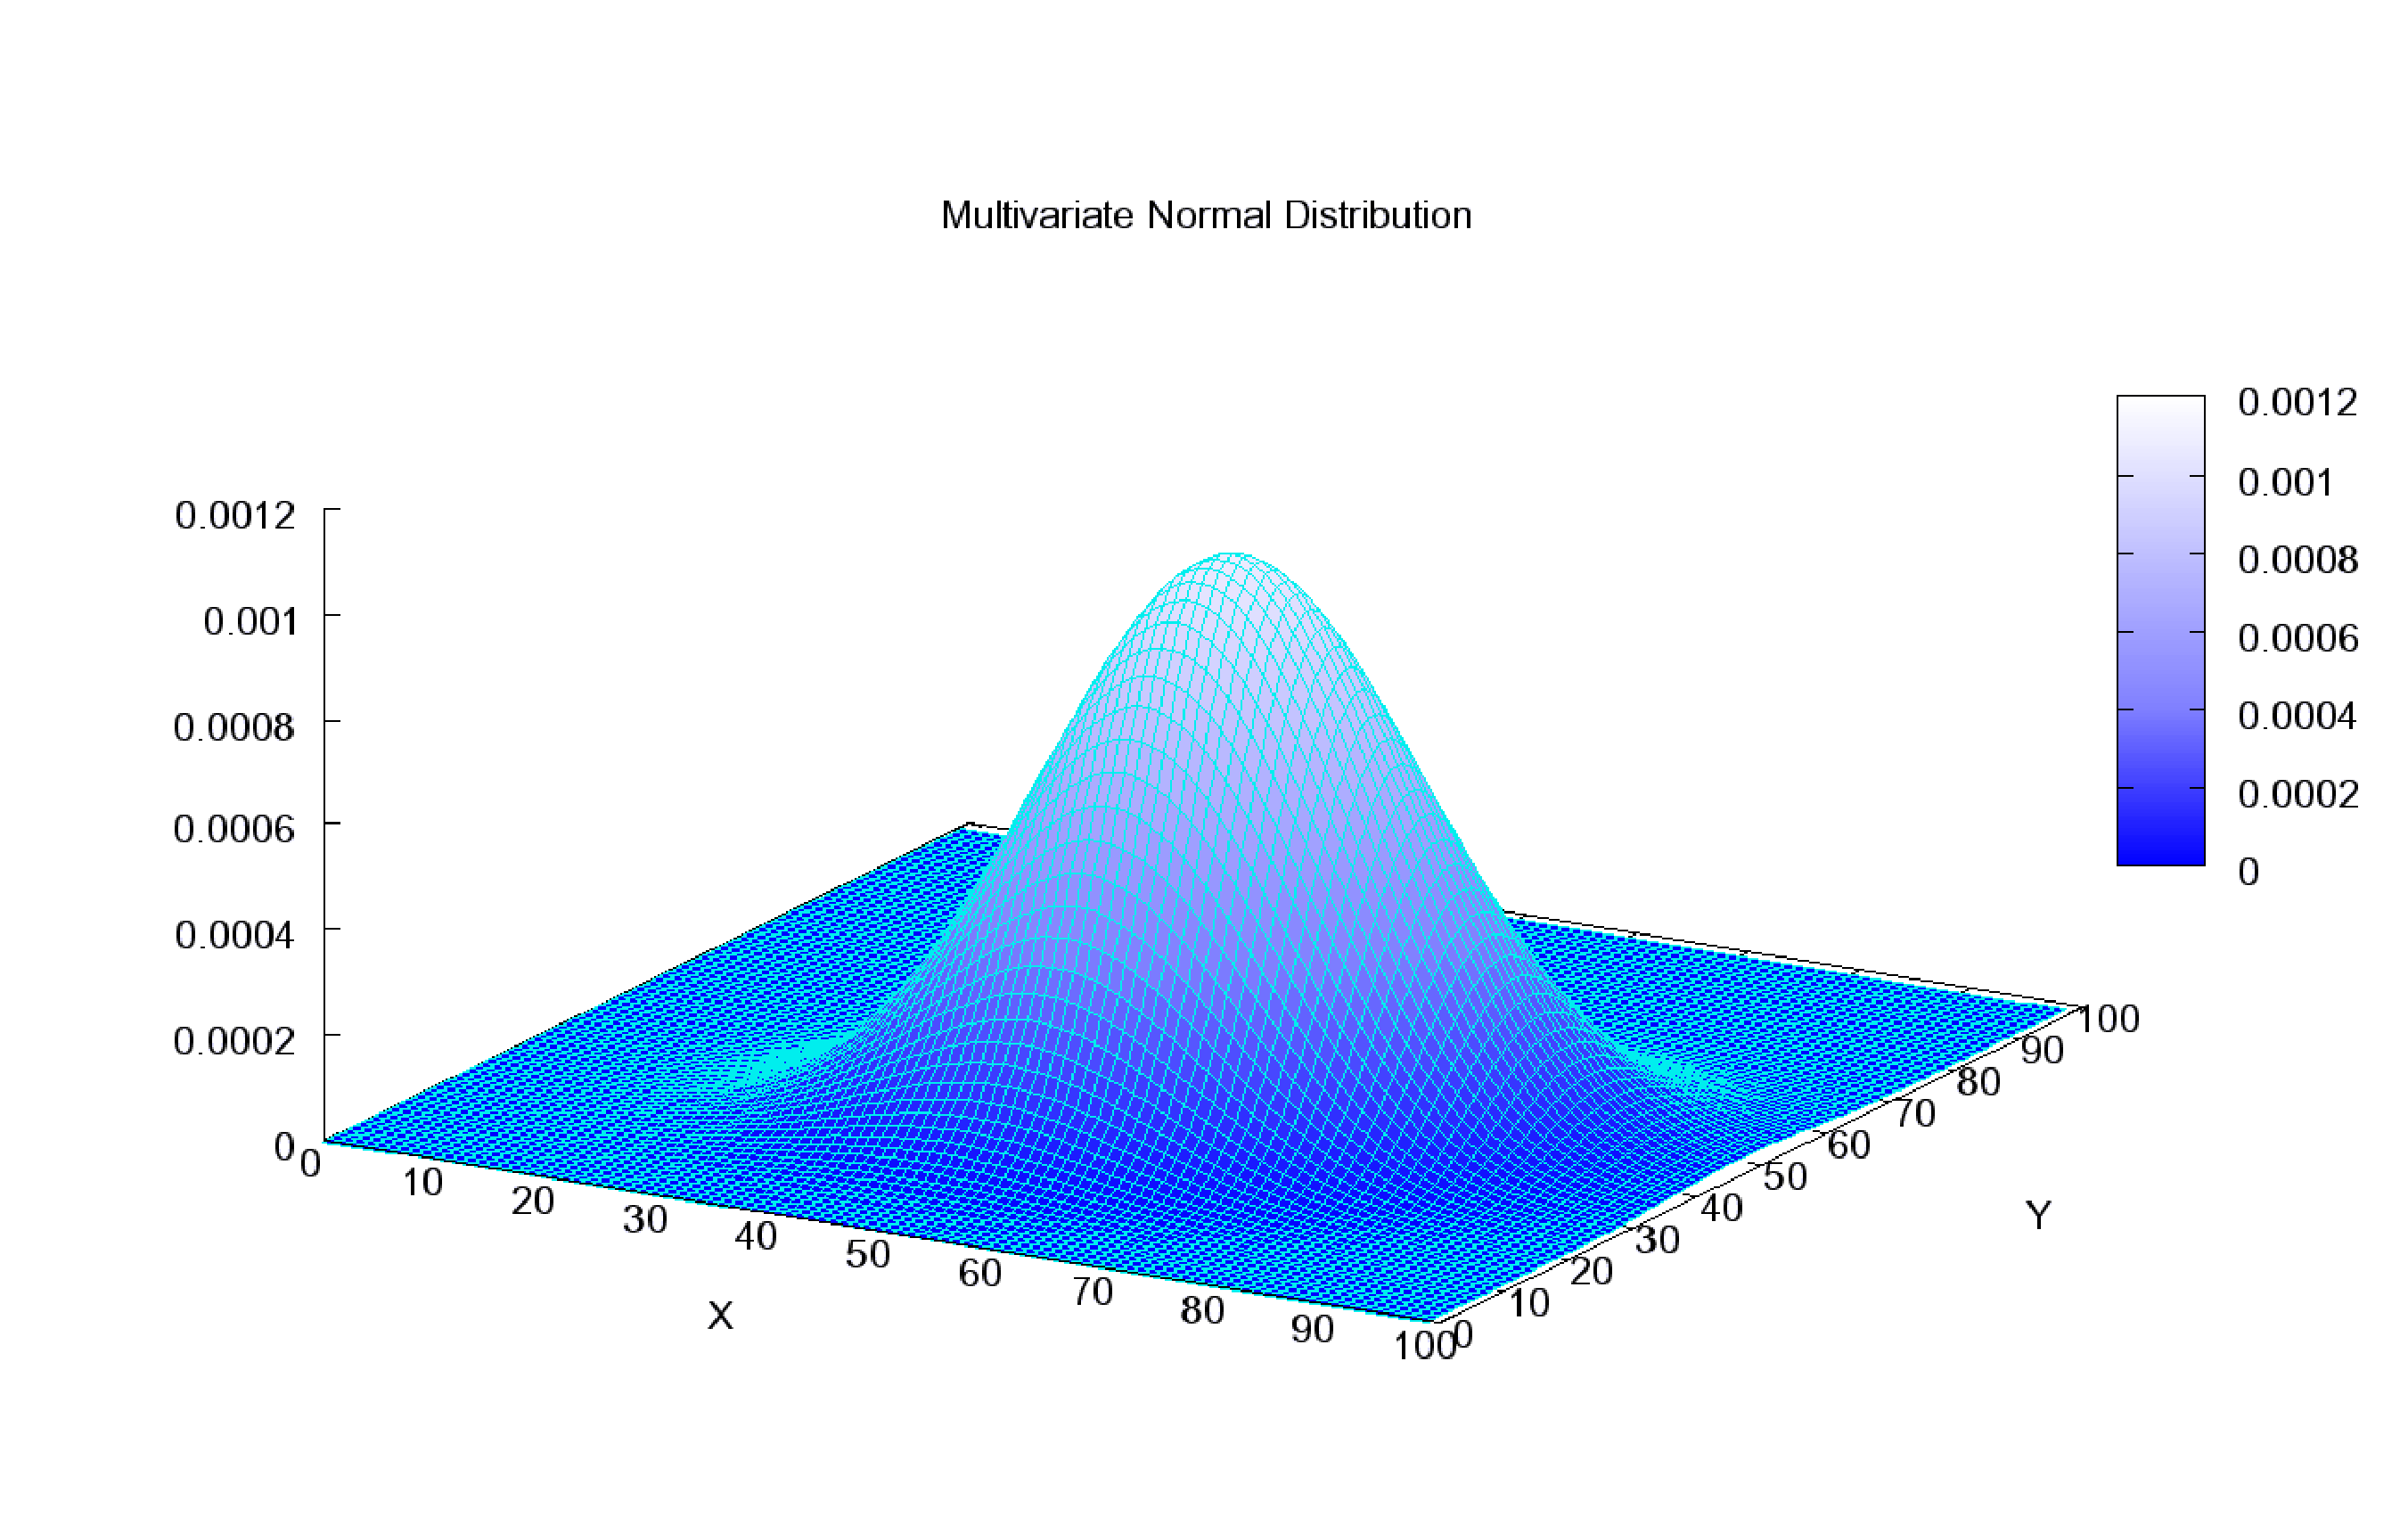
\includegraphics[width=1.0\columnwidth]{figures/mv_gaussian.eps}
    \caption{Bivariate Gaussian function}
    \label{fig:mv_gaussian}
  \end{center}
\end{figure}

In the multivariate case, the properties ariund the sum and the linear operation also fulfill: 
\begin{itemize}
 \item $\tilde{\mathbf{z}}=\mathbf{A}\tilde{\mathbf{x}} \ 
      \rightarrow \tilde{\mathbf{z}}=\mathcal{N}(\mathbf{A}\boldsymbol\mu_x,\mathbf{A}\mathbf{C}_x\mathbf{A}^T)$, 
      where $\mathbf{A}\in \mathbb{R}^{m \times n}$.
 \item $\tilde{z}=\tilde{x}+\tilde{y} \ 
      \rightarrow \tilde{z}=\mathcal{N}(\mu_x+\mu_y,\sqrt{\sigma^2_x+\sigma^2_y})$
\end{itemize}


\subsection{Gaussian Uncertainty Propagation}
How uncertainty is propagated through different physical or computing processes is a major topic in robotics, specially in perception, but also in precise actuation. Specifically, we are interested in know how a density function reshapes due to some computation, view point change, ...

In previous subsections we've seen that Gaussian random variables and vectors have the great property that it is easy (not only conceptually but also computationally) to compute their parameters once they pass through linear operations (product by scalar and sum). We've also seen in section~\ref{sec:Linearization} that non-linear functions can be linearized, by assuming a linearization error. Therefore, linearization and Gaussian uncertainty propagation are two operations very common in many robotics algorithms. At intuitive level, linearization remains valid as long as uncertainty is enough \textit{small} with respect to how the function changes (indicated by Jacobian). 

\paragraph{Example \theexamplecounter. Vehicle frames revisited (with uncertainty)}
\stepcounter{examplecounter}
Let's come back to example presented in subsection~\ref{subsec:homogeneous_matrix}. However, now we will focus only in the system vehicle-sensor-point, but we will introduce several uncertainty sources. First of all, the point~$q$ is reported by a sensor in polar coordinates $(q_r,q_{\alpha})$. The datasheet of of that sensor indicates standard deviations for range measurement and azimuth~$\sigma_r$ and~$\sigma_{\alpha}$ respectively. So the covariance matrix of a point~$q$ at the measurement space $(r,\alpha)$ is:
\begin{equation}
 \mathbf{C}^{r\alpha}_q = 
 \left[
 \begin{array}{cc}
 \sigma^2_r & 0                \\
 0          & \sigma^2_{\alpha} \\
 \end{array}
 \right]
\end{equation}
Point~$q$ in the homogeneous space, with respect to the sensor frame, is computed as:
\begin{equation}
\left[
\begin{array}{c}
    \mathbf{q}_S\\
    1 \\
 \end{array}
\right]
=
 \left[
 \begin{array}{c}
 q^S_x \\
 q^S_y \\
 1
 \end{array}
 \right]
  =
 \left[
 \begin{array}{c}
 q_r \cos \alpha \\
 q_r \sin \alpha \\
 1
 \end{array}
 \right]
\end{equation}
The equation above is not linear in the random variable, $[r\ \alpha]^T$, so to propagate the uncertainty from the measurement space $(r\alpha)$, to the homogeneous one $(xy1)$, we have to linearize this equation. From the section~\ref{sec:Linearization}, we learned that multivariate functions required the Jacobian to be computed in order to linearize the function around a point of interest, $(q_r,q_{\alpha})$:
\begin{equation}
 \mathbf{J}_{r\alpha} = 
 \left[
 \begin{array}{cc}
 \cos \alpha  & -r\sin \alpha \\
 \sin \alpha  &  r\cos \alpha \\
 0	      & 0	      \\
 \end{array}
 \right]
\end{equation}
Once we know the (approximative) linear relation between~$q^S$ and~$q^{r\alpha}$, we can propagate the uncertainty by using the properties of how Gaussian ranodm variables modify through linear systems, as discussed in subsection~\ref{subsec:mulivariate_gaussian_distribution}:
\begin{equation}
 \mathbf{C}^S_q = \mathbf{J}_{r\alpha}\mathbf{C}^{r\alpha}_q\mathbf{J}_{r\alpha}^T
\end{equation}
where the Jacobian has to be evaluated at the point~$(q^r,q^{\alpha})$. Thereafter, we want to compute the uncertain point~$q$ with respect to the vehicle frame. At this frame, the point is affected by two sources of uncertainty:
\begin{itemize}
 \item Propagation of the uncertainty of $q^S$ to the new frame~$(\mathbf{C}^{B1}_q)$.
 \item New uncertainty introduced by calibration innaccuracies of sensor mounting point on-board the vehicle~$(\mathbf{C}^{B2}_q)$.
\end{itemize}
So the final covariance matrix of the point, with respect to the vehicle frame, would be like the sum of two contributions:
\begin{equation}
 \mathbf{C}^{B}_q = \mathbf{C}^{B1}_q + \mathbf{C}^{B2}_q
\end{equation}
Let's start computing $\mathbf{C}^{B1}_q$. Recalling to the example in subsection~\ref{subsec:homogeneous_matrix}, the point~$\mathbf{q}^S$ is expressed with respect to the vehicle frame as:
\begin{equation}
\left[
 \begin{array}{c}
  \mathbf{q}^B\\
  1 \\
 \end{array}
\right] 
= 
\mathbf{T}^B_S 
\left[
\begin{array}{c}
    \mathbf{q}_S\\
    1 \\
 \end{array}
\right];\\
\end{equation}
so in that case, the relation is linear with the random variable~$q^S$, so we can apply directly the covariance propagation equation without having to linearize:
\begin{equation}
 \mathbf{C}^{B1}_q = \mathbf{T}^B_S \mathbf{C}^S_q (\mathbf{T}^B_S)^T
\end{equation}
The second term of the equation was related to errors in the calibration mounting pose (point and orientation) of the sensor withe respect to the vehicle. This errors are assumed to follow a Gaussian distribution and the three variables involved are considered to be unrelated between them, so the covariance matrix modelling this calibration error looks like:
\begin{equation}
 \mathbf{C}^B_S = 
 \left[
 \begin{array}{ccc}
 \sigma^2_{m_x} & 0 & 0  \\
 0 & \sigma^2_{m_y} & 0 \\
 0 & 0 & \sigma^2_{\beta} \\
 \end{array}
 \right]
\end{equation}
where $\sigma_{m_x},\sigma_{m_y}$ and~$\sigma_{\beta}$ are the standard deviations of the mounting pose components~$(m_x,m_y,m_{\beta})$. But in that case, point~$\mathbf{q}^B$ is not linear with respect this new random variable~$(m_x,m_y,m_{\beta})$. The relation was:
\begin{equation}
 \mathbf{q}^B =
 \left[
 \begin{array}{ccc}
  \cos\beta & -\sin\beta & m_x \\
  \sin\beta & \cos\beta & m_y \\
  0 & 0 & 1
 \end{array}
 \right]
 \left[
 \begin{array}{c}
  q^S_x \\
  q^S_y \\
  1
 \end{array}
 \right]
 = 
 \left[
 \begin{array}{c}
  q^S_x\cos\beta - q^S_y\sin\beta + m_x \\
  q^S_x\sin\beta + q^S_y\cos\beta + m_y \\
  1
 \end{array}
 \right]
\end{equation}
which is clearly a non-linear relation of~$\mathbf{q}^B$ with respect to the sensor mounting pose $(m_x,m_y,\beta)$, even if it is linear with respect to~$\mathbf{q}^S$ (as it was exploited to compute $\mathbf{C}^{B1}_q$). Thus, we know that to face non-linear relations, we have to linearize, by computing the Jacobian matrix with respect to the non-linear dependencies:
\begin{equation}
 \mathbf{J}_{m\beta} = 
 \left[
 \begin{array}{ccc}
 1 & 0 & -q^S_x\sin\beta - q^S_y\cos\beta  \\
 0 & 1 &  q^S_x\cos\beta - q^S_y\sin\beta \\
 0 & 0 & 0
 \end{array}
 \right]
\end{equation}
and now, we are capable to propagate the uncertainty of the calibration errors to the point coordinates in the vehicle frame: 
\begin{equation}
 \mathbf{C}^{B2}_q = \mathbf{J}_{m\beta}\mathbf{C}^S_q\mathbf{J}_{m\beta}^T
\end{equation}
So the final covariance matrix of the point~$\mathbf{q}$ with respect to the vehicle frame is:
\begin{equation}
 \mathbf{C}^{B}_q = \mathbf{C}^{B1}_q + \mathbf{C}^{B2}_q = 
    \mathbf{T}^B_S \mathbf{C}^S_q (\mathbf{T}^B_S)^T 
    + 
    \mathbf{J}_{m\beta}\mathbf{C}^S_q\mathbf{J}_{m\beta}^T
\end{equation}

The ScuiuLab code below implements all this example and plots the ellispes related to~$\mathbf{C^S_q}$ and~$\mathbf{C^B_q}$.
\begin{mdframed}
\tiny
\begin{verbatim} 
 //clear
clear;

//include files (where draw_ellispes_from_cov() function is defined)
exec("/home/andreu/dev/uncertainty_propagation/ellipsesAxis.sci");

//Sensor point q detection in polar coordinates (r,a) (measurement space)
r_q = 8;
a_q = 23*%pi/180; //rad  (20.467)
qS = [r_q*cos(a_q); r_q*sin(a_q);1]; //point q in homogeneous coordinates wrt to the Sensor

//sensor noise in polar coordinates (measurement space) 
sigma_range = 0.03; //meters 
sigma_angle = 0.1*%pi/180; //rad 
Cra_q = [sigma_range^2 0;0 sigma_angle^2]; //covariance matrix in measurement space
J_ra = [cos(a_q) -r_q*sin(a_q); sin(a_q) r_q*cos(a_q); 0 0]; //Jacobian: Linearization from measurement to homogeneous space

//Sensor mounting point with respect to the vehicle base
betaB_S = 35*%pi/180; //orientation angle of the sensor wrt the base
mB_S = [31;12]; //xy coordinates of the sensor wrt the base
RB_S = [cos(betaB_S) -sin(betaB_S); sin(betaB_S) cos(betaB_S)]; //rotation of the sensor wrt the base (R base2sensor)
TB_S = [RB_S mB_S;0 0 1]; //homogeneous transform of the sensor wrt the base (T base2sensor)

//sensor mounting point uncertainty (calibration error, or on-line sensor frame positioning error)
sigma_mx = 0.005; //meters
sigma_my = 0.005; //meters
sigma_beta = 0.1*%pi/180; //rad
C_mbeta = [sigma_mx^2 0 0; 0 sigma_my^2 0; 0 0 sigma_beta^2];
J_mbeta = [1 0 -qS(1)*sin(betaB_S)-qS(2)*cos(betaB_S); 0 1 qS(1)*cos(betaB_S)-qS(2)*sin(betaB_S); 0 0 0];

//------------------ PROPAGATE COVARIANCES --------------
CS_q = J_ra*Cra_q*J_ra'; disp(CS_q);
CB_q = TB_S*CS_q*TB_S' + J_mbeta*C_mbeta*J_mbeta'; disp(CB_q);

//------------------- DRAW ELLIPSES ---------------------
figure('BackgroundColor',[1 1 1]);
drawaxis();
ph = gca(); // handle
ph.isoview = 'on';
ph.axes_visible = ["on","on","off"]
ph.grid = [1,1];
ph.auto_scale="on";
ph.auto_clear = 'off';

//CS_q
draw_ellispes_from_cov([0 0], CS_q(1:2,1:2),ph);
e=gce(); // get the current entity (the last created, the ellipses)
set(e,"foreground",1);
set(e,"thickness",3);
ph.auto_clear = 'off';

//CB_q
draw_ellispes_from_cov([0 0], CB_q(1:2,1:2),ph);
e=gce(); // get the current entity (the last created, the ellipses)
set(e,"foreground",2);
set(e,"thickness",3);
\end{verbatim}
\end{mdframed}
For the values of the code example above, the two plotted ellipses are shown in Figure~\ref{fig:ellipses}. In the black ellispes related to the point uncertainty with respect to the sensor frame,~$\mathbf{C^S_q}$, it can be seen how the shape of the uncertainty is larger in the range measurement component~($r$), rather than in the angular measurement~($\alpha$). The blue ellispes shows the effect of a rotation provoked by the frame transformation ($\mathbf{T}^B_S$), but also the growing due to a new source of uncertainty due to errors on teh calibration mounting pose. 
\begin{figure}[bth!]
  \begin{center}
    
\includegraphics[width=1.0\columnwidth]{figures/ellipses.eps}
    \caption{Ellises related to covariance matrixes~$\mathbf{C^S_q}$ (black) and~$\mathbf{C^B_q}$ (blue).}
    \label{fig:ellipses}
  \end{center}
\end{figure}







\newpage
\section{Linear System Solving}
\subsection{Unweighted Linear Least Squares}
\subsection{Weighted Linear Least Squares}

\section{Kinematics and Dynamics}
About how coordinate frames move according their velocities, rotational rates, positions and orientations. 

\subsection{Wheel Kinematics}
Cases of Wheeled platforms

\subsection{Dynamics}
Coriolis: cases: Feature point, people tracking, ...

\section{Odometry}
2D and 3D twist integration

\section{State Estimation}
KF, EKF, PF, Optimization, ...


\bibliographystyle{plain}
\bibliography{../../../papers/bib_references/references}

\end{document}
